%! TEX root = ../dsa-review.tex

For a string $T$, substring of $T$ is denoted by $T[i,j]$ where $0 \leq i \leq j < M$.

\begin{description}
  \item[Prefix] Substring from $0$ to $i$ where $i < M$
  \item[Suffix] Substring from $i$ to $M - 1$ where $i \geq 0$
\end{description}

\section{Brute-force String Pattern Matching}

Suppose we want to check if a string $P$ (stands for "pattern") is a substring of a longer string $T$.
If you are lazy, you can use the following brute-force pattern-matching algorithm.

\begin{minted}{python}
  def bruteForceMatch(T, P):  # P is the "pattern" string we wish to find in T
      n, m = len(T), len(P)
      for i in range(n - m):
          j = 0
          while j < m and T[i + j] == P[j]:
              j += 1
          if j == m:
              return i

      return -1
\end{minted}

\noindent The algorithm goes through $T$ and checks compares characters of $P$ until we reach the end $P$, returning the earliest match.
The algorithm is highly inefficient, taking $O(nm)$ time in the worst case scenario.

\begin{center}
  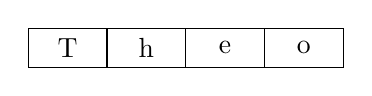
\begin{tikzpicture}
    \node [draw, minimum width=1cm, minimum height=0.5cm] at (0, 1) {T};
    \node [draw, minimum width=1cm, minimum height=0.5cm] at (1, 1) {h};
    \node [draw, minimum width=1cm, minimum height=0.5cm] at (2, 1) {e};
    \node [draw, minimum width=1cm, minimum height=0.5cm] at (3, 1) {o};
  \end{tikzpicture}

  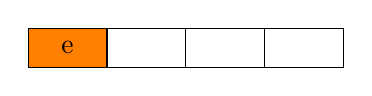
\begin{tikzpicture}
    \node [draw, minimum width=1cm, minimum height=0.5cm, fill=orange] at (0, 1) {e};
    \node [draw, minimum width=1cm, minimum height=0.5cm] at (1, 1) {};
    \node [draw, minimum width=1cm, minimum height=0.5cm] at (2, 1) {};
    \node [draw, minimum width=1cm, minimum height=0.5cm] at (3, 1) {};
  \end{tikzpicture}

  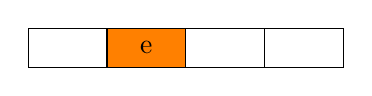
\begin{tikzpicture}
    \node [draw, minimum width=1cm, minimum height=0.5cm] at (0, 1) {};
    \node [draw, minimum width=1cm, minimum height=0.5cm, fill=orange] at (1, 1) {e};
    \node [draw, minimum width=1cm, minimum height=0.5cm] at (2, 1) {};
    \node [draw, minimum width=1cm, minimum height=0.5cm] at (3, 1) {};
  \end{tikzpicture}

  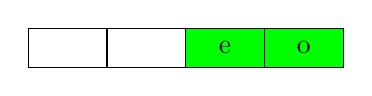
\begin{tikzpicture}
    \node [draw, minimum width=1cm, minimum height=0.5cm] at (0, 1) {};
    \node [draw, minimum width=1cm, minimum height=0.5cm] at (1, 1) {};
    \node [draw, minimum width=1cm, minimum height=0.5cm, fill=green] at (2, 1) {e};
    \node [draw, minimum width=1cm, minimum height=0.5cm, fill=green] at (3, 1) {o};
  \end{tikzpicture}
\end{center}

\section{KMP Algorithm}

Knuth-Morris-Pratt algorithm is an efficient pattern matching algorithm with $O(n + m)$ time complexity.

\noindent It uses the pre-computed \textsc{LPS} (Longest Proper Prefix, where proper prefix is a prefix of $T$ that does not include $T$ itself) array.
The name \textsc{LPS} is slightly misleading, as what \textsc{Failure} function is actually calculating is \textbf{the length of the longest matching prefix \& suffix for each substring}.

\begin{minted}{python}
  def failure(pattern):
      m = len(pattern)
      lps = [0] * m
      j = 0
      for i in range(1, m):
          while j > 0 and pattern[i] != pattern[j]:
              j = lps[j - 1]
          if pattern[i] == pattern[j]:
              j += 1
          lps[i] = j

      return lps
\end{minted}

\noindent For example, for the string \textsc{"ababcab"}, the \textsc{Failure} function produces the following result.

\begin{align*}
  &\mathrm{lps} = \mathrm{failure}(``ababcab'') \\
  &\mathrm{lps}[0] = 0 & (``a'') \\
  &\mathrm{lps}[1] = 0 & (``ab") \\
  &\mathrm{lps}[2] = 1 & (``\mathbf{\overline{a}}b\mathbf{\overline{a}}") \\
  &\mathrm{lps}[3] = 2 & (``\mathbf{\overline{ab}}\ \mathbf{\overline{ab}}") \\
  &\mathrm{lps}[4] = 0 & (``ababc") \\
  &\mathrm{lps}[5] = 1 & (``\mathbf{\overline{a}}babc\mathbf{\overline{a}}") \\
  &\mathrm{lps}[6] = 2 & (``\mathbf{\overline{ab}}abc\mathbf{\overline{ab}}")
\end{align*}

\noindent The \textsc{KMP} driver function uses the \textsc{LPS} array to find the earliest index where the pattern is found.

\begin{minted}{python}
  def kmp(T, pattern):
      n, m = len(T), len(pattern)
      lps = failure(T, pattern)
      i, j = 0, 0
      while i < n:
          if T[i] == pattern[j]:
              if j == m - 1:
                  return i - j
              else:
                  i += 1
                  j += 1
          elif j > 0:
              j = lps[j - 1]
          else:
              i += 1
      return -1
\end{minted}

\begin{center}
  \colorbox{white}{\makebox(9,9){\textcolor{black}{a}}}
  \colorbox{white}{\makebox(9,9){\textcolor{black}{b}}}
  \colorbox{white}{\makebox(9,9){\textcolor{black}{a}}}
  \colorbox{white}{\makebox(9,9){\textcolor{black}{b}}}
  \colorbox{white}{\makebox(9,9){\textcolor{black}{c}}}
  \colorbox{white}{\makebox(9,9){\textcolor{black}{a}}}
  \colorbox{white}{\makebox(9,9){\textcolor{black}{a}}}
  \colorbox{white}{\makebox(9,9){\textcolor{black}{b}}}
  \colorbox{white}{\makebox(9,9){\textcolor{black}{a}}}
  \colorbox{white}{\makebox(9,9){\textcolor{black}{c}}}
  \colorbox{white}{\makebox(9,9){\textcolor{black}{c}}}
  \colorbox{white}{\makebox(9,9){\textcolor{black}{a}}}
  \colorbox{white}{\makebox(9,9){\textcolor{black}{b}}}
  \colorbox{white}{\makebox(9,9){\textcolor{black}{a}}}
  \colorbox{white}{\makebox(9,9){\textcolor{black}{b}}}
  \colorbox{white}{\makebox(9,9){\textcolor{black}{c}}}
  \colorbox{white}{\makebox(9,9){\textcolor{black}{a}}}
  \colorbox{white}{\makebox(9,9){\textcolor{black}{b}}}
  \\
  \colorbox{green}{\makebox(9,9){\textcolor{black}{a}}}
  \colorbox{green}{\makebox(9,9){\textcolor{black}{b}}}
  \colorbox{green}{\makebox(9,9){\textcolor{black}{a}}}
  \colorbox{green}{\makebox(9,9){\textcolor{black}{b}}}
  \colorbox{green}{\makebox(9,9){\textcolor{black}{c}}}
  \colorbox{green}{\makebox(9,9){\textcolor{black}{a}}}
  \colorbox{orange}{\makebox(9,9){\textcolor{black}{b}}}
  \colorbox{white}{\makebox(9,9){\textcolor{black}{}}}
  \colorbox{white}{\makebox(9,9){\textcolor{black}{}}}
  \colorbox{white}{\makebox(9,9){\textcolor{black}{}}}
  \colorbox{white}{\makebox(9,9){\textcolor{black}{}}}
  \colorbox{white}{\makebox(9,9){\textcolor{black}{}}}
  \colorbox{white}{\makebox(9,9){\textcolor{black}{}}}
  \colorbox{white}{\makebox(9,9){\textcolor{black}{}}}
  \colorbox{white}{\makebox(9,9){\textcolor{black}{}}}
  \colorbox{white}{\makebox(9,9){\textcolor{black}{}}}
  \colorbox{white}{\makebox(9,9){\textcolor{black}{}}}
  \colorbox{white}{\makebox(9,9){\textcolor{black}{}}}
  \\
  Since the length of longest prefix/suffix is 1 (\textsc{``a''}), start matching at index 1.
  \\
  \colorbox{gray}{\makebox(9,9){\textcolor{black}{}}}
  \colorbox{gray}{\makebox(9,9){\textcolor{black}{}}}
  \colorbox{gray}{\makebox(9,9){\textcolor{black}{}}}
  \colorbox{gray}{\makebox(9,9){\textcolor{black}{}}}
  \colorbox{gray}{\makebox(9,9){\textcolor{black}{}}}
  \colorbox{cyan}{\makebox(9,9){\textcolor{black}{a}}}
  \colorbox{orange}{\makebox(9,9){\textcolor{black}{b}}}
  \colorbox{white}{\makebox(9,9){\textcolor{black}{}}}
  \colorbox{white}{\makebox(9,9){\textcolor{black}{}}}
  \colorbox{white}{\makebox(9,9){\textcolor{black}{}}}
  \colorbox{white}{\makebox(9,9){\textcolor{black}{}}}
  \colorbox{white}{\makebox(9,9){\textcolor{black}{}}}
  \colorbox{white}{\makebox(9,9){\textcolor{black}{}}}
  \colorbox{white}{\makebox(9,9){\textcolor{black}{}}}
  \colorbox{white}{\makebox(9,9){\textcolor{black}{}}}
  \colorbox{white}{\makebox(9,9){\textcolor{black}{}}}
  \colorbox{white}{\makebox(9,9){\textcolor{black}{}}}
  \colorbox{white}{\makebox(9,9){\textcolor{black}{}}}
  \\
  Since the length of longest prefix/suffix is 0, start matching at index 0.
  \\
  \colorbox{gray}{\makebox(9,9){\textcolor{black}{}}}
  \colorbox{gray}{\makebox(9,9){\textcolor{black}{}}}
  \colorbox{gray}{\makebox(9,9){\textcolor{black}{}}}
  \colorbox{gray}{\makebox(9,9){\textcolor{black}{}}}
  \colorbox{gray}{\makebox(9,9){\textcolor{black}{}}}
  \colorbox{gray}{\makebox(9,9){\textcolor{black}{}}}
  \colorbox{green}{\makebox(9,9){\textcolor{black}{a}}}
  \colorbox{green}{\makebox(9,9){\textcolor{black}{b}}}
  \colorbox{green}{\makebox(9,9){\textcolor{black}{a}}}
  \colorbox{orange}{\makebox(9,9){\textcolor{black}{b}}}
  \colorbox{white}{\makebox(9,9){\textcolor{black}{}}}
  \colorbox{white}{\makebox(9,9){\textcolor{black}{}}}
  \colorbox{white}{\makebox(9,9){\textcolor{black}{}}}
  \colorbox{white}{\makebox(9,9){\textcolor{black}{}}}
  \colorbox{white}{\makebox(9,9){\textcolor{black}{}}}
  \colorbox{white}{\makebox(9,9){\textcolor{black}{}}}
  \colorbox{white}{\makebox(9,9){\textcolor{black}{}}}
  \colorbox{white}{\makebox(9,9){\textcolor{black}{}}}
  \\
  Since the length of longest prefix/suffix is 1 (\textsc{``a''}), start matching at index 1.
  \\
  \colorbox{gray}{\makebox(9,9){\textcolor{black}{}}}
  \colorbox{gray}{\makebox(9,9){\textcolor{black}{}}}
  \colorbox{gray}{\makebox(9,9){\textcolor{black}{}}}
  \colorbox{gray}{\makebox(9,9){\textcolor{black}{}}}
  \colorbox{gray}{\makebox(9,9){\textcolor{black}{}}}
  \colorbox{gray}{\makebox(9,9){\textcolor{black}{}}}
  \colorbox{gray}{\makebox(9,9){\textcolor{black}{}}}
  \colorbox{gray}{\makebox(9,9){\textcolor{black}{}}}
  \colorbox{cyan}{\makebox(9,9){\textcolor{black}{a}}}
  \colorbox{orange}{\makebox(9,9){\textcolor{black}{b}}}
  \colorbox{white}{\makebox(9,9){\textcolor{black}{}}}
  \colorbox{white}{\makebox(9,9){\textcolor{black}{}}}
  \colorbox{white}{\makebox(9,9){\textcolor{black}{}}}
  \colorbox{white}{\makebox(9,9){\textcolor{black}{}}}
  \colorbox{white}{\makebox(9,9){\textcolor{black}{}}}
  \colorbox{white}{\makebox(9,9){\textcolor{black}{}}}
  \colorbox{white}{\makebox(9,9){\textcolor{black}{}}}
  \colorbox{white}{\makebox(9,9){\textcolor{black}{}}}
  \\
  Since the length of longest prefix/suffix is 0, start matching at index 0.
  \\
  \colorbox{gray}{\makebox(9,9){\textcolor{black}{}}}
  \colorbox{gray}{\makebox(9,9){\textcolor{black}{}}}
  \colorbox{gray}{\makebox(9,9){\textcolor{black}{}}}
  \colorbox{gray}{\makebox(9,9){\textcolor{black}{}}}
  \colorbox{gray}{\makebox(9,9){\textcolor{black}{}}}
  \colorbox{gray}{\makebox(9,9){\textcolor{black}{}}}
  \colorbox{gray}{\makebox(9,9){\textcolor{black}{}}}
  \colorbox{gray}{\makebox(9,9){\textcolor{black}{}}}
  \colorbox{gray}{\makebox(9,9){\textcolor{black}{}}}
  \colorbox{orange}{\makebox(9,9){\textcolor{black}{a}}}
  \colorbox{white}{\makebox(9,9){\textcolor{black}{}}}
  \colorbox{white}{\makebox(9,9){\textcolor{black}{}}}
  \colorbox{white}{\makebox(9,9){\textcolor{black}{}}}
  \colorbox{white}{\makebox(9,9){\textcolor{black}{}}}
  \colorbox{white}{\makebox(9,9){\textcolor{black}{}}}
  \colorbox{white}{\makebox(9,9){\textcolor{black}{}}}
  \colorbox{white}{\makebox(9,9){\textcolor{black}{}}}
  \colorbox{white}{\makebox(9,9){\textcolor{black}{}}}
  \\
  Since the length of longest prefix/suffix is 0, start matching at index 0.
  \\
  \colorbox{gray}{\makebox(9,9){\textcolor{black}{}}}
  \colorbox{gray}{\makebox(9,9){\textcolor{black}{}}}
  \colorbox{gray}{\makebox(9,9){\textcolor{black}{}}}
  \colorbox{gray}{\makebox(9,9){\textcolor{black}{}}}
  \colorbox{gray}{\makebox(9,9){\textcolor{black}{}}}
  \colorbox{gray}{\makebox(9,9){\textcolor{black}{}}}
  \colorbox{gray}{\makebox(9,9){\textcolor{black}{}}}
  \colorbox{gray}{\makebox(9,9){\textcolor{black}{}}}
  \colorbox{gray}{\makebox(9,9){\textcolor{black}{}}}
  \colorbox{gray}{\makebox(9,9){\textcolor{black}{}}}
  \colorbox{orange}{\makebox(9,9){\textcolor{black}{a}}}
  \colorbox{white}{\makebox(9,9){\textcolor{black}{}}}
  \colorbox{white}{\makebox(9,9){\textcolor{black}{}}}
  \colorbox{white}{\makebox(9,9){\textcolor{black}{}}}
  \colorbox{white}{\makebox(9,9){\textcolor{black}{}}}
  \colorbox{white}{\makebox(9,9){\textcolor{black}{}}}
  \colorbox{white}{\makebox(9,9){\textcolor{black}{}}}
  \colorbox{white}{\makebox(9,9){\textcolor{black}{}}}
  \\
  Since the length of longest prefix/suffix is 0, start matching at index 0.
  \\
  \colorbox{gray}{\makebox(9,9){\textcolor{black}{}}}
  \colorbox{gray}{\makebox(9,9){\textcolor{black}{}}}
  \colorbox{gray}{\makebox(9,9){\textcolor{black}{}}}
  \colorbox{gray}{\makebox(9,9){\textcolor{black}{}}}
  \colorbox{gray}{\makebox(9,9){\textcolor{black}{}}}
  \colorbox{gray}{\makebox(9,9){\textcolor{black}{}}}
  \colorbox{gray}{\makebox(9,9){\textcolor{black}{}}}
  \colorbox{gray}{\makebox(9,9){\textcolor{black}{}}}
  \colorbox{gray}{\makebox(9,9){\textcolor{black}{}}}
  \colorbox{gray}{\makebox(9,9){\textcolor{black}{}}}
  \colorbox{gray}{\makebox(9,9){\textcolor{black}{}}}
  \colorbox{green}{\makebox(9,9){\textcolor{black}{a}}}
  \colorbox{green}{\makebox(9,9){\textcolor{black}{b}}}
  \colorbox{green}{\makebox(9,9){\textcolor{black}{a}}}
  \colorbox{green}{\makebox(9,9){\textcolor{black}{b}}}
  \colorbox{green}{\makebox(9,9){\textcolor{black}{a}}}
  \colorbox{green}{\makebox(9,9){\textcolor{black}{a}}}
  \colorbox{green}{\makebox(9,9){\textcolor{black}{b}}}
\end{center}

\noindent Okay, kind of a bad example, here is a simpler example with $T = abacaabaccabacab$ and $P = abacab$.

\begin{align*}
  &\mathrm{lps} = \mathrm{failure}(``abacab'') \\
  &\mathrm{lps}[0] = 0 & (``a'') \\
  &\mathrm{lps}[1] = 0 & (``ab") \\
  &\mathrm{lps}[2] = 1 & (``\mathbf{\overline{a}}b\mathbf{\overline{a}}") \\
  &\mathrm{lps}[3] = 0 & (``abac") \\
  &\mathrm{lps}[4] = 1 & (``\mathbf{\overline{a}}bac\mathbf{\overline{a}}") \\
  &\mathrm{lps}[5] = 2 & (``\mathbf{\overline{ab}}ac\mathbf{\overline{ab}}") \\
\end{align*}

\begin{center}
  \colorbox{white}{\makebox(9,9){\textcolor{black}{a}}}
  \colorbox{white}{\makebox(9,9){\textcolor{black}{b}}}
  \colorbox{white}{\makebox(9,9){\textcolor{black}{a}}}
  \colorbox{white}{\makebox(9,9){\textcolor{black}{c}}}
  \colorbox{white}{\makebox(9,9){\textcolor{black}{a}}}
  \colorbox{white}{\makebox(9,9){\textcolor{black}{a}}}
  \colorbox{white}{\makebox(9,9){\textcolor{black}{b}}}
  \colorbox{white}{\makebox(9,9){\textcolor{black}{a}}}
  \colorbox{white}{\makebox(9,9){\textcolor{black}{c}}}
  \colorbox{white}{\makebox(9,9){\textcolor{black}{c}}}
  \colorbox{white}{\makebox(9,9){\textcolor{black}{a}}}
  \colorbox{white}{\makebox(9,9){\textcolor{black}{b}}}
  \colorbox{white}{\makebox(9,9){\textcolor{black}{a}}}
  \colorbox{white}{\makebox(9,9){\textcolor{black}{c}}}
  \colorbox{white}{\makebox(9,9){\textcolor{black}{a}}}
  \colorbox{white}{\makebox(9,9){\textcolor{black}{b}}}
  \\
  \colorbox{green}{\makebox(9,9){\textcolor{black}{a}}}
  \colorbox{green}{\makebox(9,9){\textcolor{black}{b}}}
  \colorbox{green}{\makebox(9,9){\textcolor{black}{a}}}
  \colorbox{green}{\makebox(9,9){\textcolor{black}{c}}}
  \colorbox{green}{\makebox(9,9){\textcolor{black}{a}}}
  \colorbox{orange}{\makebox(9,9){\textcolor{black}{b}}}
  \colorbox{white}{\makebox(9,9){\textcolor{black}{}}}
  \colorbox{white}{\makebox(9,9){\textcolor{black}{}}}
  \colorbox{white}{\makebox(9,9){\textcolor{black}{}}}
  \colorbox{white}{\makebox(9,9){\textcolor{black}{}}}
  \colorbox{white}{\makebox(9,9){\textcolor{black}{}}}
  \colorbox{white}{\makebox(9,9){\textcolor{black}{}}}
  \colorbox{white}{\makebox(9,9){\textcolor{black}{}}}
  \colorbox{white}{\makebox(9,9){\textcolor{black}{}}}
  \colorbox{white}{\makebox(9,9){\textcolor{black}{}}}
  \colorbox{white}{\makebox(9,9){\textcolor{black}{}}}
  \\
  Since the length of longest prefix/suffix is 1 (\textsc{``a''}), start matching at index 1.
  \\
  \colorbox{gray}{\makebox(9,9){\textcolor{black}{}}}
  \colorbox{gray}{\makebox(9,9){\textcolor{black}{}}}
  \colorbox{gray}{\makebox(9,9){\textcolor{black}{}}}
  \colorbox{gray}{\makebox(9,9){\textcolor{black}{}}}
  \colorbox{cyan}{\makebox(9,9){\textcolor{black}{a}}}
  \colorbox{orange}{\makebox(9,9){\textcolor{black}{b}}}
  \colorbox{white}{\makebox(9,9){\textcolor{black}{}}}
  \colorbox{white}{\makebox(9,9){\textcolor{black}{}}}
  \colorbox{white}{\makebox(9,9){\textcolor{black}{}}}
  \colorbox{white}{\makebox(9,9){\textcolor{black}{}}}
  \colorbox{white}{\makebox(9,9){\textcolor{black}{}}}
  \colorbox{white}{\makebox(9,9){\textcolor{black}{}}}
  \colorbox{white}{\makebox(9,9){\textcolor{black}{}}}
  \colorbox{white}{\makebox(9,9){\textcolor{black}{}}}
  \colorbox{white}{\makebox(9,9){\textcolor{black}{}}}
  \colorbox{white}{\makebox(9,9){\textcolor{black}{}}}
  \\
  Since the length of longest prefix/suffix is 0, start matching at index 0.
  \\
  \colorbox{gray}{\makebox(9,9){\textcolor{black}{}}}
  \colorbox{gray}{\makebox(9,9){\textcolor{black}{}}}
  \colorbox{gray}{\makebox(9,9){\textcolor{black}{}}}
  \colorbox{gray}{\makebox(9,9){\textcolor{black}{}}}
  \colorbox{gray}{\makebox(9,9){\textcolor{black}{}}}
  \colorbox{green}{\makebox(9,9){\textcolor{black}{a}}}
  \colorbox{green}{\makebox(9,9){\textcolor{black}{b}}}
  \colorbox{green}{\makebox(9,9){\textcolor{black}{a}}}
  \colorbox{green}{\makebox(9,9){\textcolor{black}{c}}}
  \colorbox{orange}{\makebox(9,9){\textcolor{black}{a}}}
  \colorbox{white}{\makebox(9,9){\textcolor{black}{}}}
  \colorbox{white}{\makebox(9,9){\textcolor{black}{}}}
  \colorbox{white}{\makebox(9,9){\textcolor{black}{}}}
  \colorbox{white}{\makebox(9,9){\textcolor{black}{}}}
  \colorbox{white}{\makebox(9,9){\textcolor{black}{}}}
  \colorbox{white}{\makebox(9,9){\textcolor{black}{}}}
  \\
  Since the length of longest prefix/suffix is 0, start matching at index 0.
  \\
  \colorbox{gray}{\makebox(9,9){\textcolor{black}{}}}
  \colorbox{gray}{\makebox(9,9){\textcolor{black}{}}}
  \colorbox{gray}{\makebox(9,9){\textcolor{black}{}}}
  \colorbox{gray}{\makebox(9,9){\textcolor{black}{}}}
  \colorbox{gray}{\makebox(9,9){\textcolor{black}{}}}
  \colorbox{gray}{\makebox(9,9){\textcolor{black}{}}}
  \colorbox{gray}{\makebox(9,9){\textcolor{black}{}}}
  \colorbox{gray}{\makebox(9,9){\textcolor{black}{}}}
  \colorbox{gray}{\makebox(9,9){\textcolor{black}{}}}
  \colorbox{orange}{\makebox(9,9){\textcolor{black}{a}}}
  \colorbox{white}{\makebox(9,9){\textcolor{black}{}}}
  \colorbox{white}{\makebox(9,9){\textcolor{black}{}}}
  \colorbox{white}{\makebox(9,9){\textcolor{black}{}}}
  \colorbox{white}{\makebox(9,9){\textcolor{black}{}}}
  \colorbox{white}{\makebox(9,9){\textcolor{black}{}}}
  \colorbox{white}{\makebox(9,9){\textcolor{black}{}}}
  \\
  Since the length of longest prefix/suffix is 0, start matching at index 0.
  \\
  \colorbox{gray}{\makebox(9,9){\textcolor{black}{}}}
  \colorbox{gray}{\makebox(9,9){\textcolor{black}{}}}
  \colorbox{gray}{\makebox(9,9){\textcolor{black}{}}}
  \colorbox{gray}{\makebox(9,9){\textcolor{black}{}}}
  \colorbox{gray}{\makebox(9,9){\textcolor{black}{}}}
  \colorbox{gray}{\makebox(9,9){\textcolor{black}{}}}
  \colorbox{gray}{\makebox(9,9){\textcolor{black}{}}}
  \colorbox{gray}{\makebox(9,9){\textcolor{black}{}}}
  \colorbox{gray}{\makebox(9,9){\textcolor{black}{}}}
  \colorbox{gray}{\makebox(9,9){\textcolor{black}{}}}
  \colorbox{green}{\makebox(9,9){\textcolor{black}{a}}}
  \colorbox{green}{\makebox(9,9){\textcolor{black}{b}}}
  \colorbox{green}{\makebox(9,9){\textcolor{black}{a}}}
  \colorbox{green}{\makebox(9,9){\textcolor{black}{c}}}
  \colorbox{green}{\makebox(9,9){\textcolor{black}{a}}}
  \colorbox{green}{\makebox(9,9){\textcolor{black}{b}}}
\end{center}

\noindent Okay, that was also not a good example, but hope you get the gist; when a failure in matcing occurs, KMP algorithm skips searching the part where the prefix and suffix is known to match.

\section{Trie}

\section{PATRICIA}

\section{Huffman Coding}
